\documentclass[../Proposed Method.tex]{subfiles}
\begin{document}

% \textbf{What are technical indicators}
Technical indicators are the rule of thumb or pattern-based signals produced mathematically by the stock price or volume. The fundatioin of technical indicators is the historical prices of the stocks. It is belived that the history will repeated itself as the time extends. In other words, patterns of the market behavior continously appears throughout the history of the stock market. By analyzing the historical data, technical analysis use indicators to determine the timing to buy or sell stocks.

\subsubsection{Moving Average (MA)}

% \textbf{What is Moving Average}
A Moving Average is an indicator that shows the trend of stock price of a company. If the moving average was decreasing, it indicates that the price is falling recently. If the moving average was increasing, it indicates that the price is rising recently. There are several different types of moving averages. The most popular one is the Simple Moving Average (SMA), which is the indicator that is used in this research. The main difference between the moving averages is that the weighting applies to the price of stocks when calculating the indicator.

\bigbreak

% \textbf{SMA formula}
SMA is the average closed price of a certain period of time (e.g., 5 days). The period of days that is been used to calculate the averge price is called look-back period. Among all the MA, SMA is an indicator that can be easily calculated, because the weight, which applies to the price of stocks when calculating SMA is equally weighted. The formula of SMA is shown in \ref{SMA}, where $N$ is the look-back period and $T$ is the date of today.

\begin{equation}
    \label{SMA}
    \scalebox{1}
    {$SMA_{N} = \dfrac{price_{T-N}+price_{T-N+1}+price_{T-N+2}+...+price_{T-2}+price_{T-1}}{N}$}
\end{equation}

% \textbf{How to use MA}
The most common way to use MA is to compare the relationship between two MA trends, known as crossover. The way to define a crossover is that when plotting two different MA values, the first MA line crosses through the second MA line from the bottom. This is also referred to as a golden cross. On the other hand, a death cross is that when the first MA line crosses through the second MA line of from above. We can simplify the trading strategy of using these two MA into MA($MA_{1},\ MA_{2}$). Table \ref{trad_MA} shows the parameters of traditional MA that are frequently been use by investers. The combination of the traditional strategy is restricted. Only two types of strategies are allowed, MA(Short-term, Mid-term), MA(Mid-term, Long-term). Hence there are 8 strategies in traditional MA.

\begin{table}[H]
    \centering
    \captionsetup{font={footnotesize}}
    \caption{Tradition MA strategies}
    \label{trad_MA}
    \footnotesize
    \begin{tabularx}{0.8\textwidth}{c @{\extracolsep{\fill}} cc}
        \toprule
        \textbf{Short-term} & \textbf{Mid-term}      & \textbf{Long-term}   \\
        \midrule
        5 days (one week)   & 20 days (one month)    & 120 days (half year) \\
        10 days (two weeks) & 60 days (three months) & 240 days (one year)  \\
        \bottomrule
    \end{tabularx}
\end{table}

% \begin{table}[ht]
%     \centering
%     \captionsetup{font={footnotesize}}
%     \caption{Tradition MA strategies}
%     \label{trad_MA}
%     \footnotesize
%     \begin{tabular*}{0.8\textwidth}{c @{\extracolsep{\fill}} cc}
%         \toprule
%         \textbf{Short-term}  & \textbf{Mid-term}      & \textbf{Long-term}   \\
%         \midrule
%         5 days (one week)   & 20 days (one month)    & 120 days (half year) \\
%         10 days (two weeks) & 60 days (three months) & 240 days (one year)  \\
%         \bottomrule
%     \end{tabular*}
% \end{table}

% \begin{table}
%     \centering
%     \captionsetup{font={footnotesize}}
%     \caption{Tradition MA strategies}
%     \label{trad_MA}
%     \footnotesize
%     \resizebox{0.5\textwidth}{!}{%
%         \begin{tabular}{ccc}
%             \toprule
%             \textbf{Short-term}  & \textbf{Mid-term}      & \textbf{Long-term}   \\
%             \midrule
%             5 days (one week)   & 20 days (one month)    & 120 days (half year) \\
%             10 days (two weeks) & 60 days (three months) & 240 days (one year)  \\
%             \bottomrule
%         \end{tabular}%
%     }
% \end{table}

% \begin{table}
%     \centering
%     \captionsetup{font={footnotesize}}
%     \caption{Tradition MA strategies}
%     \label{trad_MA}
%     \footnotesize
%     \begin{tabularx}\linewidth{ccc}
%         \toprule
%         \textbf{Short-term}  & \textbf{Mid-term}      & \textbf{Long-term}   \\
%         \midrule
%         5 days (one week)   & 20 days (one month)    & 120 days (half year) \\
%         10 days (two weeks) & 60 days (three months) & 240 days (one year)  \\
%         \bottomrule
%     \end{tabularx}%
% \end{table}

Figure \ref{cross_demo} demostrate the timimg of golden cross and death cross when using SMA(5, 20). A buy signal is triggered when a golden cross appears. A selling signal is triggered when a death cross appears. These two types of crossover are the important signal to determine the timing of buying or selling the stocks.

\begin{figure}[H]
    \centering
    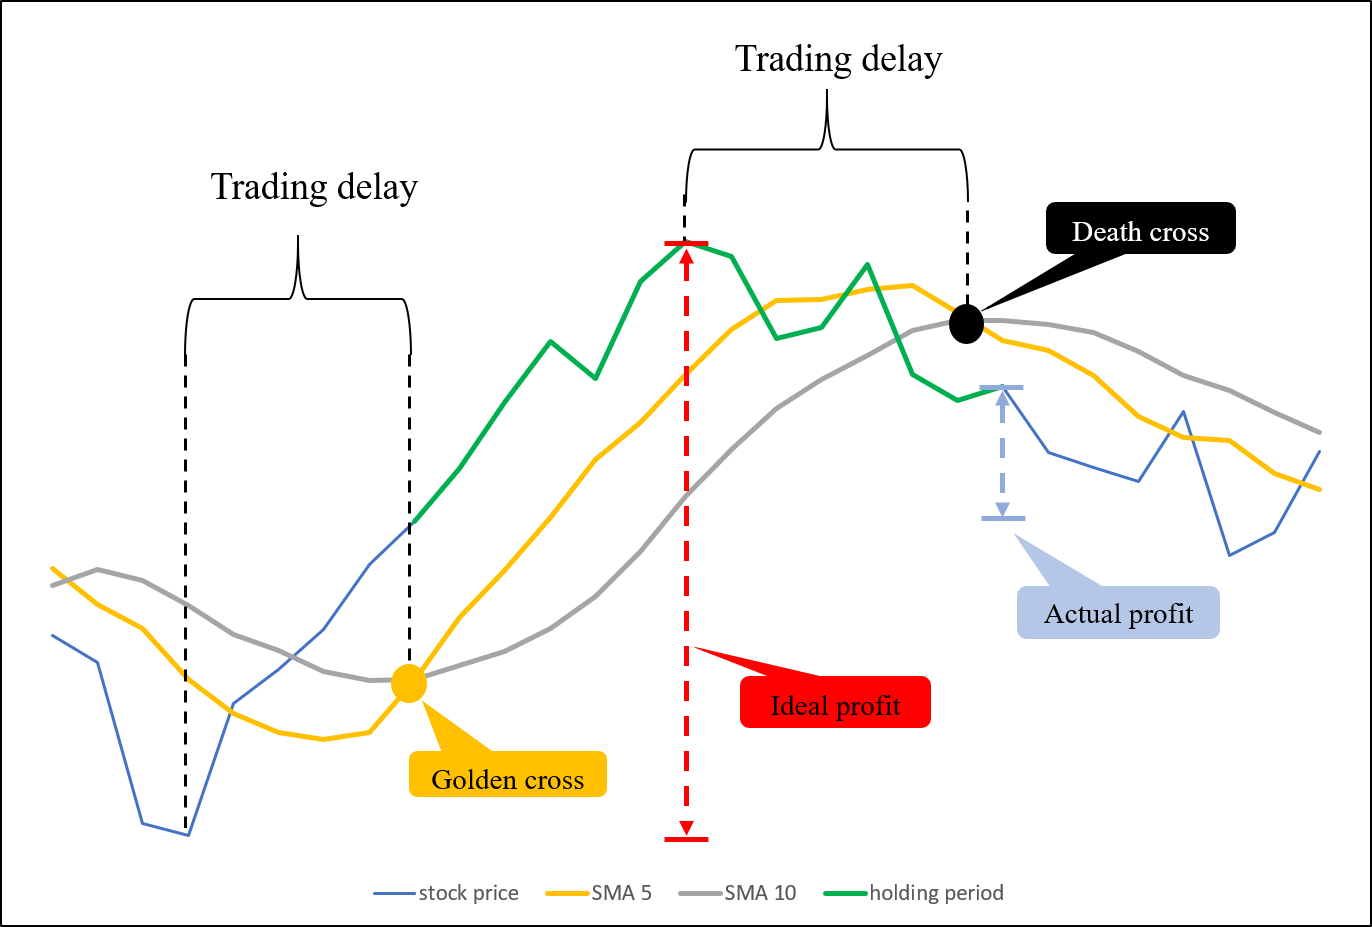
\includegraphics[scale = 0.6] {figure/cross1.png}
    \captionsetup{font={footnotesize}}
    % \vspace{-3em}
    \caption{Demostration of using strategy SMA(5, 20)}
    % \vspace{-0.5em}
    \label{cross_demo}
\end{figure}

% \textbf{Characteristics of MA}inconsistentparameters
Even though MA is a popular investment indicator, there are still some downsides. The first issue is that moving average is a lagging indicator. As we can see in figure \ref{cross_demo}, the golden cross and death cross are lagging behind the best time to buy or sell shares, leading to lower profits. The second issue is that there are too few traditional strategies. It is difficult to make a profit with just those few strategies. The third problem has to do with the lack of parameters. MA uses just two parameters to find the golden cross and the death cross. Using the same parameters to buy and sell does not appear to be sufficient.

\bigbreak

In order to break the boundaries of traditional MA strategy and find more accuate buying and selling point, this study extends the parameters of MA. There will be four parameters, two for buying and two for selling, rather than jus two for buying and selling. In addition, the parameters can be selected from 1 to 256, instead of choosing from short-term, mid-term and long-term.
This significantly increases the number of strategies from 8 to $\text{256}^\text{4}$. More than 4.2 billion strategies that can be select when using MA as indicator. Comparison of MA traditoinal strategy and new MA strategy are shown in table \ref{trad_and_GN_SMA}.

\begin{table}[H]
    \centering
    \captionsetup{font={footnotesize}}
    \caption{Comparison of SMA traditoinal strategy and new MA strategy}
    \label{trad_and_GN_SMA}
    \footnotesize
    \def\arraystretch{1.5}
    \begin{tabularx}{0.8\textwidth}{c @{\extracolsep{\fill}} cc}
        \toprule
        \textbf{}      & \textbf{Traditoinal strategy} & \textbf{new MA strategy}                                           \\
        \midrule
        strategy       & MA($MA_1,\ MA_2$)             & MA($MA_{buy_{1}},\ MA_{buy_{2}},\ MA_{sell_{1}}, \ MA_{sell_{2}}$) \\
        solution space & 8                             & $\text{2}^\text{32}$                                               \\
        \bottomrule
    \end{tabularx}
\end{table}

\subsubsection{Relative Strength Index (RSI)}

% \textbf{What is RSI}
Relative Strength Index (RSI) is a momentum oscillator that was first introduced by J. Welles Wilder, Jr. [3] in 1978. This is a popular indicator in financial technical analysis that measures the magnitude of recent prices changes. The basic idea of RSI is to measure how quickly traders are bidding the price of the stocks up or down. RSI sees the uprising stocks as a buyer's strength, and the downswing stocks as a sellers' strength, which are referrd as overbought and oversold.

\bigbreak

% \textbf{RSI formula}
The period of days need to calculate RSI is referred as look-back period. The RSI calculation process can be split into two steps. For step one (as shown in formula \ref{step_1}), the average gain and loss is the average upward change and downward change of the stocks price during the look-back period. As for step two, with the result from step one, we can calculate the next RSI using formula \ref{step_2} recursively, where $N$ is look-back period. RSI oscillates between 0 and 100.
% The RSI formulas are as follows.

\begin{equation}
    \label{step_1}
    \scalebox{1}
    {$RSI_{step\ one}=100-\left[\dfrac{100}{1+\dfrac{Average\ gain}{Average\ loss}}\right]$}
    % \vspace{1em}
\end{equation}

\begin{equation}
    \label{step_2}
    \scalebox{1}
    {$RSI_{step\ two}=100-\left[\dfrac{100}{1+\dfrac{Previous\ Average\ Gain\times(N-1)+Current\ Gain}{-(Previous\ Average\ Loss)\times(N-1)+Current\ Loss}}\right]$}
    % \vspace{1em}
\end{equation}

% \textbf{How to use RSI}
When using RSI, there are three parameters: look-back period, overbought, and oversold. First, select the period of days to calculate RSI. Second, choose the thresholds for oversold and overbought, which means that when RSI meets these thresholds, it will trigger the buy or sell signal. The representation of a RSI strategy is RSI ($period$) ($oversold,\ overbought$). Traditionally, RSI is mostly used on a 14-day timeframeand for look-back period according to Wilder and is considered oversold when below 30 and overbought when above 70. Most of the investors use 6, 5, or 14 as a look-back period, and oversold and overbought are (30, 70), (20, 80), where the sum of these two parameters is equal to 100. The frequently used parameters of traditional strategies are shown in table \ref{trad_RSI}.

\begin{table}[H]
    \centering
    \captionsetup{font={footnotesize}}
    \caption{Tradition RSI strategies}
    \label{trad_RSI}
    \footnotesize
    \begin{tabularx}{0.25\textwidth}{c @{\extracolsep{\fill}} cc}
        \toprule
        \textbf{period} & \textbf{(oversold, overbought)} \\
        \midrule
        5               & (20, 80)                        \\
        6                                                 \\
        14              & (30, 70)                        \\
        \bottomrule
    \end{tabularx}
\end{table}

% \textbf{Characteristics of RSI}
The traditional strategies restrict the probability to find the perfect time to buy or sell stocks. However, this research extends the look-back periods from 1 to 256, oversold and overbought from 0 to 100, and the sum of oversold and overbought does not necessarily need to be equal to 100. For example, RSI(100)(47, 89) or RSI(9)(19, 55), etc. After removing the restriction of traditional strategies, the potential of RSI has been unlocked. There is a great chance to find a strategy which can better adaptive to the every changing stock markets. The comparison of RSI traditoinal strategy and new RSI strategy is chown in table \ref{trad_and_GN_RSI}.

\begin{table}[H]
    \centering
    \captionsetup{font={footnotesize}}
    \caption{Comparison of RSI traditoinal strategy and new RSI strategy}
    \label{trad_and_GN_RSI}
    \footnotesize
    \def\arraystretch{1.5}
    \begin{tabular*}{0.8\textwidth}{c @{\extracolsep{\fill}} cc}
        \toprule
        \textbf{}&\textbf{Traditoinal strategy}  & \textbf{new RSI strategy}  \\
        \midrule
        strategy & RSI (5 or 6 or 14) and (20, 80) or (30, 70) & RSI (1 to 256) (0 to 127, 0 to 127)  \\
        solution space & 6 & $\text{2}^\text{22}$  \\
        \bottomrule
    \end{tabular*}
\end{table}

\end{document}